%% Example data sheet
%% Feel free to modify and use this file for any purpose, under
%% either the LaTeX Project Public License or under public domain.

% Options here are passed to the article class.
% Most common options: 10pt, 11pt, 12pt
\documentclass[10pt]{datasheet}

% Input encoding and typographical rules for English language
\usepackage[utf8]{inputenc}
\usepackage[english]{babel}
\usepackage[english]{isodate}

% tikz is used to draw images in this example, but you can
% also use \includegraphics{}.
\usepackage{tikz}
\usepackage{pgfplots}
\usepackage{circuitikz}
\usetikzlibrary{calc}

% These define global texts that are used in headers and titles.
\title{ETL Tamale Module Design}
\author{ETL Module design team}
\date{June 2022}
\revision{Revision 1}
\companylogo{\Huge CMS}

\begin{document}
\maketitle

\section{Features}

\begin{itemize}
\item{TBD}
\item{TBD}
\item{TBD}
\end{itemize}

\section{General Description}
TBD TBD

% Switch to next column
\vfill\break

\begin{figure}[h]
    \begin{circuitikz}[european]
        \node[op amp] (amp1) {};
        \node[op amp, below = 0.5cm, xscale = -1] (amp2) {};
        \draw (amp1.out) |- (amp2.-);
        \draw (amp2.-) ++(0, 0.3cm) node[circ]{} to +(2,0) node[above left]{5};
        \draw (amp2.out) to (amp1.+);
        \draw (amp1.+) ++(0, -0.3cm) node[circ]{} to +(-2,0) node[above right]{2};
        \draw (amp1.-) to +(-2,0) node[above right]{1};
        \draw (amp2.+) to +(2,0) node[above left]{4};
        \draw (amp1.out) +(0,0.5cm) node (Vdd) {$\mathrm{V_{DD}}$};
        \draw (Vdd.east) to +(1.5,0) node [above left]{6};
        \draw (amp2.out) +(0,-0.5cm) node (Vss) {$\mathrm{V_{SS}}$};
        \draw (Vss.west) to +(-1.6,0) node [above right]{3};
        \draw ($(amp1.north west) + (-0.5,0.5)$) rectangle ($(amp2.south west) + (0.5,-0.5)$);
    \end{circuitikz}
    \caption{Pinout and internal circuit}
\end{figure}

\begin{figure}[h]
    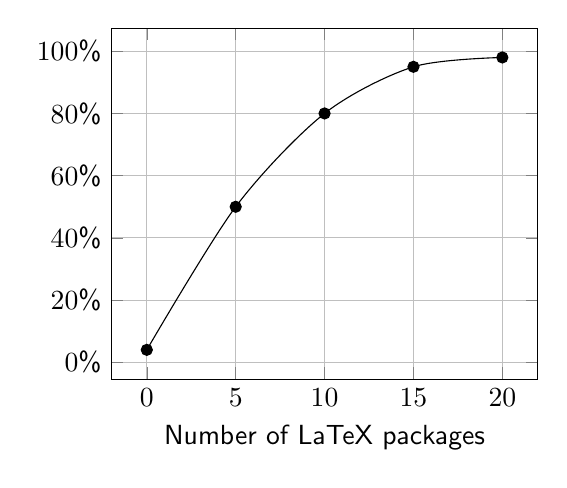
\begin{tikzpicture}
        \sffamily
        \begin{axis}[
            width=7cm,
            xlabel={Number of LaTeX packages},
            ytick distance=20,
            yticklabel={\pgfmathprintnumber{\tick}\%},
            xmajorgrids, ymajorgrids]
        \addplot[smooth,mark=*] plot coordinates {
            (0,4)
            (5,50)
            (10,80)
            (15,95)
            (20,98)
        };
        \end{axis}
    \end{tikzpicture}
    \caption{Typical data sheet production efficiency}
\end{figure}

% For wide tables, a single column layout is better. It can be switched
% page-by-page.
\onecolumn

\section{Overview of Design}

The ETL Module is built from a stack-up of a components as illustrated in Fig. \ref{fig:overview}. Starting from the bottom, the layers are:

\begin{itemize}
	\item A ceramic baseplate. Currently Alumina is the preferred material for its high thermal conductivity and relatively low cost compared to alternatives.
	\item An adhesive film. The leading candidate is an 80um thick silicone-based phase-change material. It serves as both a strong mechanical and low-resistance thermal interface between the silicon components and the baseplate.
	\item Four ETROC+LGAD subassemblies. These will be bump-bonded by an external vendor.
	\item A 2nd adhesive film. It will be the same material as the sensor-mount film, but cut to slightly different from the previous film.
	\item A PCB. This serves as the power and I/O interface between the readout board and the module via two board-to-board connectors. It also serves as a location to place any SMT passive components that must be placed very near the ETROCs.
\end{itemize}

The overall module dimensions are 56.5mm long by 43.1mm wide with an estimated stackup height of 2.97mm. For prototype modules to be constructed using ETROC2, the length is increased by 1mm to 57.5mm to ease the wirebonding process.


\begin{figure}[h]
	\includegraphics[width=\textwidth]{figures/overview.png}
	\caption{Stackup of ETL Module design}
	\label{fig:overview}
\end{figure}

This document is structured to follow the gantry-based assembly procedure while providing relevant details on the mechanical structure of the module and components along the way. A mechanical jig-based assembly is also being developed to be deployed as module factories that do not have gantries. The modules produced with either method will be identical.


\section{Module PCB}

Assembly begins with the Module PCB as the base layer of the stackup. It is important to note that the modules are built "upside down", i.e. PCB-side down, while they will be mounted baseplate-side down.

The Module PCB's dimensions match that of the module overall at 56.5x43.1mm. It has four 2.2mm diameter mounting holes, one in each corner. These are through holes for M2 screws that will serve to hold the assembly of the readout board and its several modules to the disc. They are centered 1.75mm from each edge. The PCB will be a 4-layer board with 0.5mm nominal thickness. The board-to-board connectors are JAE Electronics WP7B-S050VA1-R8000. These are surface-mount connectors with 50 connections each and an overall stacking height of 0.7mm. They are placed with a separation of 23.53mm centered on the top of the board. The top of the board will also potentially have a small number of surface-mount passive components as required by the ETROC.

The opposite side of the board has a pattern of wire-bonding pads to connect with the ETROCs. The current proposal for this pattern is illustrated in Fig. \ref{fig:wirebonding-pattern}.

\begin{figure}[h]
    \includegraphics[width=\textwidth]{figures/wirebonding-pattern.png}
    \caption{Proposed wirebonding pattern for the ETROC}
    \label{fig:wirebonding-pattern}	
\end{figure}

\section{Sensor-mount film}

As mentioned in the introduction, a set of adhesive films are used to mechanically attach the module layers together as well as provide a thermal path for removing heat from the ETROC and LGAD. The leading candidate material is Laird TPCM (Thermal Phase Change Material) 580(CHECK THIS). The film will be cut to shape by an outside vendor and will arrive to the module factories with plastic liners on each side with tabs to allow easy removal.

The sensor-mount film matches the envelope of the four ETROCs on the module. The dimensions are 42.6x46.6mm and 80um thick. The film will be applied to the Module PCB using a mechanical jig for alignment and to minimize the presence of trapped air between the film and the PCB.


\section{ETROC \& LGAD Subassembly}


\section{Wirebonding}


\section{Wirebond Encapsulation}


\section{Ahesive Films}



\section{Baseplate}

The baseplate 







\end{document}


